\chapter{Analytical Study}
\label{chp:suggested-solution}

In this chapter we'll walk through how the problem can be modelled as a multi-commodity flow problem and solved using linear programming.


\section{Modelling}

With some prior knowledge of graph algorithms, the first stab at solving the problem might be to look at our sample topologies and see a certain similarity to a max-flow problem -- edges have capacities, there's a set of sources, a set of sinks, and we want to maximize \emph{something}. However, there's a couple of things that make it hard to solve directly as a traditional flow problem, particularly that we don't have a single source and a single sink, but lots of them. Trying to model it as a single-source, single-sink problem quickly leads us to discover the limitations of that model, where we realize that if we actually solved it, how would we be able to tell which node is generating flow on a given edge? Clearly, we need a way to distinguish node A's video from node B's video. And we need to make sure that all nodes receive video from every other node, not just maximum bitrate of \emph{any} video.

If we change perspective slightly, we see that this is not a single flow problem, but a \emph{series} of flow problems, sharing an underlying constrained resource. There's the problem of routing video from A to all other nodes, there's the problem of routing video from B to all other nodes, etc. In a conversation with $n$ participants, we now have $n$ separate flow problems, which all share the same resource. However, also this model is too limiting for our use case, as video is sent at a given bitrate, and this stream can neither be split at a given node without incurring a cost, nor does it make sense to add it; two 2 Mbps videos cannot be joined to form a 4 Mbps video. If you put enough restrictions on your nodes and edges it's probable that you might be able to able to prevent this from happening, but there's another way.

This time around, imagine that we have a separate flow problem for each \emph{pair} of nodes; we have one problem routing node A's video to node B, we have one problem routing node A's video to node C, etc. This yields a total of $n(n-1)$ problems, which is $O(n^2)$. Modelling the problem this way means we don't have to add any supersinks to connect the targets; each node can act as sink for the video stream, hereafter known as the \emph{commodity}, destined for itself.

One other thing we notice from our initial graph compared to traditional flow problems is that we notice that we have \emph{node constraints} in the initial graph, while flow problems only work with \emph{edge constraints}. To accommodate this, we split each node into two parts, hereafter called the external and internal part, as illustrated in \autoref{fig:node-splitting}.

\begin{figure}
    \centering
    \begin{subfigure}[t]{.48\textwidth}
        \centering
        \includegraphics[width=\textwidth]{nodesplitting-pre}
        \subcaption{Original problem}
    \end{subfigure}
    \hfill
    \begin{subfigure}[t]{.48\textwidth}
        \centering
        \includegraphics[width=\textwidth]{nodesplitting-post}
        \subcaption{Problem after node splitting}
    \end{subfigure}
    \caption{How we can split nodes into external and internal pairs}
    \label{fig:node-splitting}
\end{figure}

As we now have a well-specified way to go from a given conversation to a graph that can be solved by max-flow algorithms, the entire problem can be solved by joining all the different subproblems under the same resource constraints, and solve as a multi-commodity max-flow problem. This class of problems can be solved with \acrfull{lp} \cite{ahuja1988network}, which can be summarized in canonical form as in \autoref{eq:lp}.

\begin{align}\label{eq:lp}
    \text{maximize}\qquad &\mathbf{c^Tx} \\
    \text{subject to}\qquad &A\mathbf{x} \leq \mathbf{b} \nonumber \\
    \text{and}\qquad &\mathbf{x} \geq \mathbf{0} \nonumber
\end{align}

The vector $\mathbf{x}$ is the variables we're trying to find a solution for, each entry in the vector defines a flow on a given edge in the graph for a given commodity. The vector $\mathbf{c}$ scores each flow to determine how much it influences the objective (hereafter known as the \emph{gain}), while the matrix $A$ and the vector $\mathbf{b}$ is the set of constraints put on the system, like staying below bandwidth, flow conversation among non-source and non-sink nodes, and so on.

As \gls{lp} is a well-known and very general technique that's effective to a vast collection of problems, there are lots of LP-solvers freely available\footnote{\url{https://en.wikipedia.org/wiki/Linear_programming\#Solvers_and_scripting_.28programming.29_languages}}. This simplifies building a solution on top of \gls{lp}; if you can model your problem as a linear program, it can be efficiently solved by existing, well-tested code. For our experimental solution we chose a solver somewhat arbitrarily among those which had Python bindings, and picked \gls{glpk}.


\section{Objective}

To approach the problem as an LP, we need to have a well-defined objective; the function the LP will try to maximize. To formulate the objective, we need to understand how several performance parameters of the system affect the QoSE.

We can start by decomposing the problem, by first looking at how to measure the QoSE from a single node's perspective to one other peer. We then aggregate all of those pairs to form the full QoSE as observed by that node, and aggregate that for all nodes in the conversation. A natural even distribution occurs here due to the \gls{wfl} and the logarithmic nature of the QoSE. If the QoSE was a linear function of performance, a small set of nodes could devour all the resources, and the QoSE would have been the same as if the resources were divided evenly. However, the logarithmic shape of the QoSE ensures that there's diminishing returns for resource consumption, thus when one node is receiving 2 Mbps, and one other is receiving 1 Mbps, increasing the latter from 1 Mbps to 2 Mbps has a greater impact on QoSE than increasing the former from 2 Mbps to 3 Mbps.

As this thesis only considers bandwidth and latency, the QoSE for a single node to a single peer will be a function of these two variables. No research was found on how these two affect the QoSE for video conversations\footnote{Much research has been done on QoS in relation to Video-on-Demand, but while the bitstream might be similar, the environment and expectations for real-time communication is entirely different from VOD, and thus not considered directly applicable in this setting}, so we'll take some grand assumptions here, and if further research is done on this topic, the model can be refined by incorpororating actual results at this step.

First, assuming that the latency is fixed, we will adopt a QoSE model from the bandwidth as given in \autoref{fig:qos-bandwidth}. The graph will be tuned to the node's device, as different devices have different saturation points for where there's nothing to gain from sending more data. Devices with larger displays and fast connections also have higher expectations to the quality of displayed video, thus the QoSE for a given bandwidth will be higher on smaller devices than large ones.

\begin{figure}
    \begin{subfigure}{.48\textwidth}
        \centering
        \begin{tikzpicture}
            \begin{axis}[
                xlabel=Bandwidth,
                width=\textwidth,
                ylabel=QoSEBandwidth,
                xmin=0,
                xmax=10,
                ymin=0,
                x axis line style={->},
                ticks=none,
                major x tick style = {opacity=1},
                minor tick length=0pt,
                axis x line=bottom,
                legend style={at={(1,0.20)}, anchor=south east,legend columns=1},
                ]

                \addplot+[domain=1:5,mark=none, color=blue]{1.5*ln(x*1.5)};
                \addlegendentry{phone}

                \addplot+[domain=1:6,mark=none, color=red]{1.3*ln(x*1.3)};
                \addlegendentry{laptop}

                \addplot+[domain=1:7,mark=none, color=black]{ln(x)};
                \addlegendentry{desktop}

                \addplot+[mark=none, color=blue] coordinates {
                    (7,3.527)
                    (10,3.527)
                };
                \addplot+[mark=none, color=red] coordinates {
                    (6,2.670)
                    (10,2.670)
                };
                \addplot+[style=solid, mark=none, color=black] coordinates {
                    (5,1.609)
                    (10,1.609)
                };
            \end{axis}
        \end{tikzpicture}
        \subcaption{QoSE as a function of bandwidth}
        \label{fig:qos-bandwidth}
    \end{subfigure}
    \hfill
    \begin{subfigure}{.48\textwidth}
        \centering
        \begin{tikzpicture}
            \begin{axis}[
                xlabel=Latency,
                width=\textwidth,
                ylabel=QoSELatency,
                xmin=0,
                xmax=10,
                ymin=0,
                x axis line style={->},
                ticks=none,
                major x tick style = {opacity=1},
                minor tick length=0pt,
                axis x line=bottom,
                legend style={at={(1,0.20)}, anchor=south east,legend columns=1},
                ]

                \addplot+[domain=2:10,mark=none, color=blue]{5-1.2^(x-2)};
                \addplot+[mark=none, color=blue] coordinates {
                    (0,4)
                    (2,4)
                };
            \end{axis}
        \end{tikzpicture}
        \subcaption{QoSE as a function of latency}
        \label{fig:qos-bandwidth}
    \end{subfigure}
    \caption{Assumed QoSE on the signal between a single pair of nodes}
    \label{fig:qos}
\end{figure}

As for latency, we assume it follows a function somewhat like the one depicted in \autoref{fig:qos-latency}. Given these two functions for QoSE, we combine them by simply adding them together, with a tunable weighting factor $w$, which says how heavily latency should count into the QoSE. When considering the QoSE as delivered to a single node, we also need to subtract the cost of using its connection, as saturating the connection will have grave impact on queueing delays and packet loss. This cost follows from the queueing delay formula, $1/(1 - \mu/\lambda)$, where $\mu$ is the capacity of the link and $\lambda$ is the offered traffic.

Formally, if we consider our flow network as a graph $G = (V, E)$, with $d_i$ as node $i$'s device. $x^c_{i,j}$ is the bandwidth of a commodity $c$ on the edge $(i,j)$, $l_{i,j}$ is the latency between nodes $i$ and $j$, and $k_{i,j}$ is the commodity from $i$ to $j$. $C$ is the set of all commodities. With $QoSEBandwidth$ and $QoSELatency$ as given in \autoref{fig:qos}, we can formulate the QoSE for the entire conversation as

\begin{gather}\label{eq:qos-pair}
    QoSEPair(i, j) = QoSEBandwidth(x_{i, j}^{k_{i, j}}, d_i) + w \times QoSELatency(l_{i,j}) \\
    QoSENode(i) = \sum_{j \in V} QoSEPair(i, j) - \sum_{c \in C} \frac{1}{u_{i,j} - x_{i,j}^{c}} \\
    QoSE = \sum_{i \in V} QoSENode(i) \label{eq:qos}
\end{gather}

\autoref{eq:qos} is then the QoSE of the entire graph, which becomes the objective function in our LP. Note that this is an assumption, more research should be conducted into finding the actual relationships involved.

This raises some other issues that has to be handled. The objective function has to be linear to be solved as a linear program, but several of its parameters are non-linear. However, all of these can be approximated arbitrarily close by piecewise linear functions, as illustrated in \autoref{fig:bitrate-quality}. This precision of the approximation can also be parametrized, as either the number of pieces to divide into or as the maximum deviation.

In the following paragraphs we'll discuss how to transform the problem to a linear one that we can solve.


\subsection{QoSE From Bandwidth}

Increasing the bitrate of video is subject to diminishing returns, increasing the bitrate from 1 Mbps to 2 Mbps yields a bigger return for the user than going from 4 Mbps to 5 Mbps. This follows from the Weber-Fechner law.

If gain from increased bandwidth was linear, increasing traffic from a given node from 4 Mbps to 5 Mbps would yield the same return as bumping another node from 1 Mbps to 2 Mbps, and thus the algorithm would be unlikely to find a fair allocation of bandwidth. Having the bandwidth gain follow a logarithmic function automatically ensures that everyone will be allocated a fair share, and still allows nodes with excess bandwidth to grow further than more constrained nodes.

To illustrate how we model this, imagine that instead of node splitting like we did above, we're doing \emph{edge splitting}, replacing a single edge connecting two nodes with a set of edges, which can have different capacities and costs. Note that we only have to split the edge coming into the node, there's nothing that affects the objective on the outgoing one. This results in a linear approximation of the actual logarithmic function, as illustrated in \autoref{fig:bitrate-quality}.

\begin{figure}
    \centering

    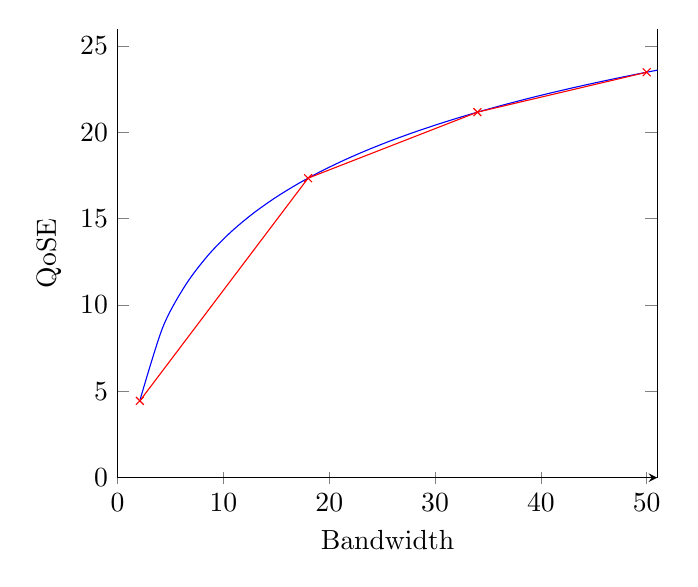
\begin{tikzpicture}
        \begin{axis}[
            xlabel={Bandwidth},
            ylabel={QoSE},
            xmin=0,
            ymin=0,
            x axis line style={->},
            axis x line=bottom,
        ]

        \addplot+[domain=0:51, mark=none, smooth]{6*ln(x)};
        \addplot+[color=red, mark=x] coordinates {
            (2.1,4.45)
            (18,17.34)
            (34,21.16)
            (50,23.47)
        };
        \end{axis}
    \end{tikzpicture}

    \caption{The logarithmic relationship between bitrate and quality (blue), and a three-part linear approximation (red)}
    \label{fig:bitrate-quality}
\end{figure}

\section{Cost of Link Utilization}

The cost of utilizing a given network link is a function of the link's utilization. We can derive this cost from the queuing delay formula,  As can be seen in \autoref{fig:utility-latency}, this function is not linear, and can thus not be used directly in our objective function. Nonetheless, we can achieve the same goal -- punishing over-utilization of individual links -- by approximating the function with a piecewise linear function. Conceptually, we can approach this in the same way as for bandwidth gains by splitting the edges into the node. Thus a 8 Mbps link might be divided into four links of 2 Mbps, with exponentially increasing costs.

Assuming that the weighting between the segments follows the queuing delay formula given above, the ratio between the extra punishment for using the last 10\% of a link and the gain from increasing bandwidth by those extra 10\% can be tuned by implementations. This ratio would basically be a measure of how heavily to hit the network to gain maximum quality. To avoid excessive packet loss, link utilization should probably not exceed 90\%, which can also be achieved by under-reporting the actual bandwidth to the algorithm. What the effects of that would be, compared to increasing the ratio towards more heavily punishing excessive link utilization, is unknown and requires more research to say anything conclusive about.

We can formulate the cost multiplier of a link as $1 + k/(\mu - \lambda)$, where $k$ is a customizable parameter for how heavily link saturation should be punished. In our experiments, $k=10$ seems appropriate. We then partition this function into a small set of piecewise linear intervals, which we can model as parallel edges between two nodes, with different capacities and costs. Keeping this set small limits the number of variables in the resulting matrix, and thus keeps processing times reasonably low.

\begin{figure}
    \centering
    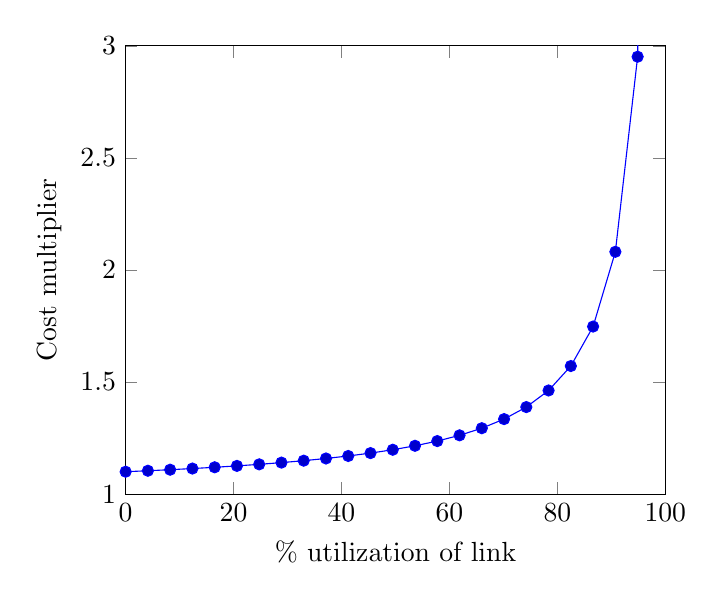
\begin{tikzpicture}
        \begin{axis}[
            xlabel={\% utilization of link},
            ylabel={Cost multiplier},
            xmin=0,
            ymin=1,
            ymax=3,
            xmax=100]

        \addplot+[domain=0:99]{1 + 10/(100 - x)};
        \end{axis}
    \end{tikzpicture}
    \caption{How packet delay grows as a function of link utilization for network links. Packet delay for us is equivalent to cost, which thus has to be approximated in an implementation.}
    \label{fig:utility-latency}
\end{figure}


\begin{center}
    \label{tab:utilization-to-cost}
    \begin{tabular}{| l | l |}
    \hline
    \textbf{Link utilization} & \textbf{Cost multiplier} \\ \hline
    0--50\% & 1.2 \\ \hline
    51--75\% & 1.40 \\ \hline
    76--80\% & 1.50 \\ \hline
    81--90\% & 2.00 \\ \hline
    \end{tabular}
\end{center}

To avoid having extra constraints to keep flowing video above a certain minimal threshold, we can replace link capacity with link \emph{slots}. A slot is the size of a minimal unit of video, like 512 kbps. This means that we only need to ensure at least one slot is used between each pair, instead of enforcing more fine-grained constraints. Using the partitioning in \autoref{tab:utilization-to-cost} as a guide, we can map any number of slots on a physical link into a set of edges $E$ in our graph where $|E| <= 4$. The number of edges to split into determines how close the approximation is, at a cost of more variables in the objective. This can be tuned by implementations.

As there's now two different edge splits on the edge between a node's internal and external parts, we have to insert a temporary node between them to separate the two edge sets.

Thus, after doing the linear approximations for both edge cost and bandwidth gains, a single node in our flow network ends up like depicted in \autoref{fig:double-edge-split}.

\begin{figure}
    \centering
    
\includegraphics[width=\textwidth]{double-edge-split}
    \caption{An example (20/5) node after two rounds of edge splitting. g is the gain from the bandwidth over an edge, c is the cost. How best to split the edges is up to implementations.}
    \label{fig:double-edge-split}
\end{figure}


\section{Alternative model}\label{sec:alternative-model}

One alternative way to model the problem, is to skip the node splitting step of the previous model, and instead connect nodes directly, but stay below bandwidth by adding constraints for the total sum going out from each node. Which model to choose is -- as in every engineering matter -- a question of priorities. The first model is a bit harder to comprehend initially, but results in fewer total edges than the latter model does when $n>3$, as can be seen in \autoref{fig:model-scaling}. Edge counts do not matter that much when $n$ is low as finding a solution will occur in trivial time anyway, but the difference might be substantial when $n$ is larger. If performance becomes an issue, more research into different ways to model the problem might yield more efficient solutions.

\begin{figure}
    \centering
    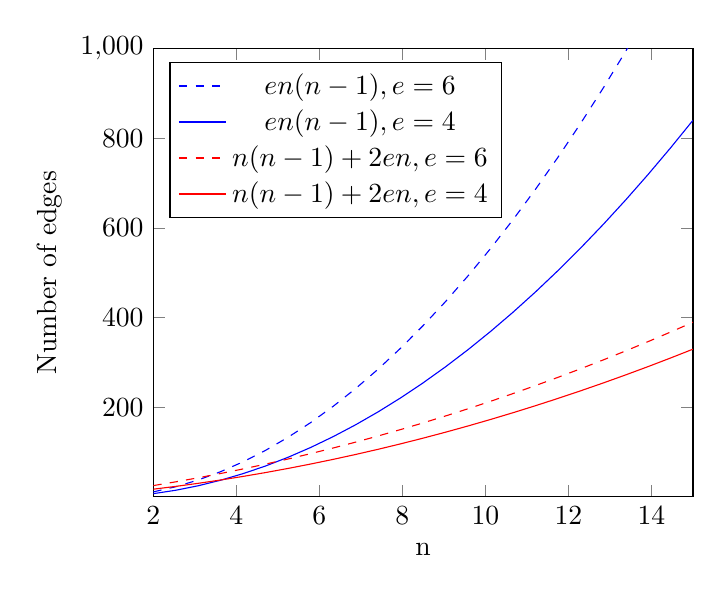
\begin{tikzpicture}
        \begin{axis}[
            xlabel={n},
            ylabel={Number of edges},
            xlabel near ticks,
            ylabel near ticks,
            legend pos=north west,
            xmin=2,
            ymin=1,
            ymax=1000,
            xmax=15,
            legend style={legend columns=1},
            minor x tick num=0,
            major x tick style = {opacity=1},
            ]

        \addplot+[dashed, domain=2:15, mark=none, color=blue]{6*x*(x-1)};
        \addlegendentry{$en(n-1), e=6$}

        \addplot+[domain=2:15, mark=none, color=blue]{4*x*(x-1)};
        \addlegendentry{$en(n-1), e=4$}

        \addplot+[dashed, domain=2:15, mark=none, color=red]{x*(x-1) + 2*x*6};
        \addlegendentry{$n(n-1) + 2en, e=6$ }

        \addplot+[domain=2:15, mark=none, color=red]{x*(x-1) + 2*x*4};
        \addlegendentry{$n(n-1) + 2en, e=4$ }
        \end{axis}
    \end{tikzpicture}
    \caption{How the number of edges in the graph scales for different modeling techniques. Blue graph is the alternative model, red is the suggested one. $e$ is the number of parallel edges to use in the linear approximations, $n$ is the size of the flow network.}
    \label{fig:model-scaling}
\end{figure}


\section{Repeaters}\label{sec:repeaters}

This is all well and good, if we solve the maximization problem given earlier we will arrive at an optimal routing of video in any graph. Using this, a browser could immediately establish flows of sustainable bitrate for everyone in the conversation, without the slow creep to steady state that is the case today. However, where today's solutions are topology-bound, we can go beyond those limitations, and use our established technique on slightly modified flow networks.

One thing we note with pure peer-to-peer topologies, is that required bandwidth in and out grows linearly with $n$, which quickly saturates constrained nodes. Going pure peer-to-peer is most often optimal in terms of latency, but if the necessary bandwidth is not available, we want to have the option to fall back to relaying some -- but not necessarily all -- nodes via some unconstrained repeater. This repeater could be provided by the service provider in a data center somewhere, or could be one of the other nodes in the conversation with excess bandwidth available\footnote{These are the nodes Skype referred to as ``supernodes'', see \cite{tree-topology-webrtc} for a study of supernodes in WebRTC.}. We have assumed that repeaters are provided in data centers for now, but the constraints can easily be adapted to accommodate nodes as repeaters in a conversation.

Formulating the constraints get a bit weird for repeaters, as they \emph{do not} conserve either bandwidth or commodities. We say that repeaters can \emph{mangle} commodities, which means it can receive the commodity $k$ sent from node A to node B, and can send it as commodity $k$ to B, but it can also send it as commodity $m$ to node C, assuming $m$ is the commodity sent by node A to node C. This is less awkward if the alternative model suggested in \autoref{sec:alternative-model} is implemented, but there was only time to implement one model for this thesis. This mangling is why we require each commodity to be received in the objective, it allows receivers to change the commodity to something else than what was sent.

There are some constraints on repeaters though, namely that the incoming amount of one commodity has to be equal to the outgoing amount of all other commodities from the same source. Practically speaking, repeaters can not change the bitrate of incoming video, either up or down. That way, a repeater is a pure IO-bound device, which does not require much else than a fast Internet connection to be operated.

Note that since commodities are routed independently in our flow network, it's possible for a node to use a repeater only for outgoing traffic, but still receive incoming traffic directly from its peers. This will probably often be the case, as many consumer connections are still highly asymmetric in inbound/outbound capacity.

Repeaters are also practical since they're not required to know the contents of the packages it forwards, and thus anyone with spare bandwidth can provide a repeater for anyone to use, without compromising the confidentiality of those conversations.

Deployment wise, repeaters are practically the same as \glspl{sfu}, thus adding repeaters to a network should not be a challenging task. The biggest difference between repeaters and SFUs is in who controls the sent data; traditional SFUs handle that themselves, negotiating with each peer which stream it should receive based on it's capabilities. Repeaters would be instructed by either the sending node or the service provider which streams should be routed where, thus a repeater is a slightly simpler unit.


\section{Transcoders}

Another unit that can be added to the flow network is a transcoder, which is like a repeater in that it has practically unconstrained bandwidth in and out, but also has the capability to transcode incoming video. If node A only has 2 Mbps upload capacity, and node B is a desktop with 10 Mbps downlink, and node C is a phone with only 1 Mbps downlink, A can send its full 2 Mbps video stream to a transcoder, which can then forward the full 2 Mbps stream to node B, but transcode the stream down to a leaner 1 Mbps stream for node C. That way A is able to fully utilize its upload capacity, while the receivers get a stream best utilizing their downlink capacity.

Transcoders are more costly to run than repeaters, due to much heavier compute operations required to transcode video in real-time. They will typically be nodes with specialized hardware for video encoding\footnote{The WebM project maintains royalty-free hardware-accelerated designs for encoding VPx: \url{http://www.webmproject.org/hardware/vp9/bige/}}.

Constraint-wise, a transcoder performs the same commodity mangling as repeaters, but can output commodities of arbitrary bitrates less than or equal to the source commodity.

However, in contrast to repeaters, transcoders have to access the contents of the calls to be able to transcode the signal. This will be the case until a homomorphic cryptosystem is available for video transcoding, which might be in a couple of years or it might be never.

Transcoders are to \glspl{mcu} what repeaters are to \glspl{sfu}; much the same, but slightly simpler.


\section{Implementation}\label{sec:implementation}

The sample implementation is in Python and uses GLPK for solving the created linear program. The script makes no attempt to optimize the creation of the linear program, thus it iterates over every single edge dozens of times. Hence, the creation of the linear program is often more expensive than the actual solving of said program. While it's true that there will always be a cost of creating the linear program, since the $O(n^4)$ objective function has to be created along with $O(n^4)$ constraints, the $n$ is usually small enough not to make the total running time unmanageable\footnote{Even with 20 nodes, $n^4$ is only 160,000 operations.}. If the approach is to be used in situations where $n$ can be large, more research is needed into optimizing this step.

The provided implementation does not fully implement everything discussed here, as time was limited. The script is capable of finding optimal routes for the objective as specified in reasonable time, but does not implement any approximation of the non-linear functions. Thus there's no punishment for maximizing network links, which means all nodes end up with 100\% utilization of their uplink, as long as someone has the capacity to receive. The script supports adding repeaters to the mix, routing video through them for nodes that are otherwise incapable of receiving video.

The script is a bit brittle in terms of adjusting parameters -- trying to tune bandwidth gain will in many cases crash it, and is thus \emph{not} recommended for any sort of production purposes.


\section{Results}\label{sec:results}

How does the approach scale with the size of the conversation? Our objective function is $O(n^4)$, the same for the number of constraints. Worst-case running time of simplex, the algorithm that powers many LP-solvers, is exponential, but is polynomial in the average case. So how do our cases fare?

\begin{figure}
    \centering
    \begin{subfigure}[t]{.48\textwidth}
        \begin{tikzpicture}
            \begin{axis}[
                xlabel=n,
                ybar stacked,
                ylabel=Execution time (s),
                xmin=2,
                xmax=10,
                ymin=0,
                width=\textwidth,
                x axis line style={->},
                axis x line=bottom,
                legend style={at={(.05,0.70)}, anchor=north west,legend columns=1},
                ]
                \input{tmp/script-runtimes}
            \end{axis}
        \end{tikzpicture}
        \subcaption{Execution times}
    \end{subfigure}
    \hfill
    \begin{subfigure}[t]{.48\textwidth}
        \begin{tikzpicture}
            \begin{axis}[
                ybar,
                xlabel=n,
                width=\textwidth,
                ylabel=Memory usage (MB),
                xmin=2,
                xmax=10,
                ymin=0,
                x axis line style={->},
                axis x line=bottom,
                ]
                \input{tmp/script-runtimes-mem}
            \end{axis}
        \end{tikzpicture}
        \subcaption{Memory usage}
    \end{subfigure}
    \caption{Resource consumption for the sample implementation on desktop computer with Intel i7 860 CPU (four cores, 2.8GHz)}
    \label{fig:script-runtimes}
\end{figure}

The script was run with a minimal video unit of 400 kbps, which allows even the weakest node in the friends case (node G, with 4 Mbps up) enough slots to stream to all other nodes. While the included script is not feature-complete, it does create test cases close to the correct size, which we can use to give some inclination to expected running time, and how it scales. The tests for 8 and 9 nodes were run by adding one and two extra nodes to the friends test case.

The best fit found for the sample data was a cubic fit\footnote{However, the quadratic fit was not much worse, at $R^2=0.9974$. The data set is small, more data is needed to say anything conclusively.}, with $R^2=0.9995$, indicating that we can expect something close to $O(n^3)$ for this approach. As mentioned earlier, since the $n$ is very small in most of the scenarious, performance is not expected to be an issue. The actual solving step took 0.4s in the 9 person case, which is far less than the actual wait today to establish a connection anyway. The time taken to build the flow network is more significant in the sample implementation, but since this is highly unoptimized Python, I expect this can be reduced substantially.
